\documentclass[11pt,a4paper]{article}

% --- packages ---
\usepackage[utf8]{inputenc}
\usepackage[T1]{fontenc}
\usepackage{lmodern}
\usepackage[english]{babel}
\usepackage{microtype}
\usepackage{amsmath, amssymb}
\usepackage[a4paper, margin=2.4cm]{geometry}
\usepackage{setspace}
\setstretch{1.05}
\usepackage{booktabs, makecell}
\usepackage{graphicx}
\usepackage{caption}
\captionsetup{font=small, labelfont=bf, skip=3pt}
\usepackage[round, sort&compress]{natbib}
\bibliographystyle{plainnat}
\usepackage{hyperref}
\hypersetup{colorlinks=true, linkcolor=black, citecolor=black, urlcolor=black}
\usepackage{xcolor}
\usepackage{titlesec}
\titleformat*{\section}{\large\bfseries}
\titleformat*{\subsection}{\normalsize\bfseries}
\titlespacing*{\section}{0pt}{8pt plus 2pt}{4pt plus 1pt}
\titlespacing*{\subsection}{0pt}{6pt plus 2pt}{2pt plus 1pt}
\titlespacing*{\paragraph}{0pt}{4pt plus 1pt}{6pt}
\setlength{\parskip}{1pt plus 1pt}
\setlength{\textfloatsep}{8pt plus 2pt minus 2pt}
\setlength{\intextsep}{8pt plus 2pt minus 2pt}
\setlength{\abovedisplayskip}{4pt plus 1pt}
\setlength{\belowdisplayskip}{4pt plus 1pt}

\title{\textbf{Generative-AI Occupational Exposure and Institutional
Trust in Europe:\\
A Within--Between Decomposition Across the European Social Survey,
2012--2024}}
\author{Karla Lučić\thanks{KU~Leuven, Master of Statistics and Data
Science. Replication code at \url{https://github.com/karlalucic/MLA}.}}
\date{April 2026}

\begin{document}
\maketitle

\begin{abstract}\noindent
Single-country studies of automation exposure and political attitudes
usually study manufacturing-heavy robot shocks. This paper asks
whether the same political-trust argument travels to the
white-collar and service-oriented GenAI exposure measured by
\citet{Gmyrek2025}. The analysis pools the European Social Survey
(R6--R11, 2012--2024; $N=165{,}969$ in 30 countries and 154
country-years), merges respondents to 4-digit ISCO-08 GenAI exposure
scores, and adds Eurostat macro indicators and OECD
employment-protection institutions. A within--between (Mundlak)
decomposition
\citep{Mundlak1978,BellJones2015,SchmidtCatranFairbrother2016}
separates two questions: do countries with higher average exposure
also have different trust levels, and do trust levels change when a
given country's exposure changes over time? The answers diverge.
The between-country coefficient is large and positive
($\hat\gamma_B = +11.24$, SE $=3.43$): high-exposure countries report
\emph{higher} institutional trust, the opposite of the
structural-grievance prediction. The within-country coefficient is
statistically indistinguishable from zero ($\hat\gamma_W = +0.02$)---a
precise null, but one estimated over the narrow band of within-country
exposure variation that remains after the common European time trend is
absorbed, so it bounds a within effect rather than ruling one out.
A Wald test rejects equality of the two slopes
($\chi^2(1)=9.66$, $p=0.002$). Education does not detectably
moderate the within-country exposure slope
($\hat{\gamma}_{W \times \mathrm{ISCED}} = -0.142$, $p=0.275$).
The evidence therefore points to a cross-sectional selection pattern:
countries with more AI-exposed occupational structures are also
richer, more service-based, and more institutionally capable. Those
country characteristics, not within-country exposure shifts, explain
the positive trust association. The pattern survives country-leverage
drops, item-by-item outcomes, dropping the COVID-disrupted R10,
leave-one-out cell aggregation, and a within-only fixed-effects
benchmark.
\end{abstract}

\section{Introduction}

The diffusion of generative AI capabilities since 2022 has reopened a
long-standing question in political sociology: do technological shocks
to the occupational structure erode trust in democratic institutions?
The empirical literature on economic dislocation answers \emph{yes}
within national borders. Trade exposure predicts support for Brexit
\citep{ColantoneStanig2018}; vulnerability to industrial robot adoption
predicts radical-right voting in Western Europe
\citep{AnelliColantoneStanig2021}; and robot installations track voting
shifts in U.S.\ counties \citep{FreyBergerChen2018}. The shared mechanism
is \emph{structural grievance}: technology displaces workers, and
displaced workers express political dissatisfaction
\citep{GidronHall2017,Kurer2020}.

Two features of this evidence base leave the question open for
generative AI. \emph{First}, the dominant exposure measures were built
for manufacturing-heavy automation
\citep{Felten2021,Webb2020,AcemogluRestrepo2020}, but generative AI
exposure concentrates in white-collar and service work
\citep{Gmyrek2025}. The political meaning of dislocation in
administration, retail, and knowledge work need not match that of
robot-driven manufacturing decline. \emph{Second}, almost all of the
existing studies are single-country. That design identifies effects
sharply within a national institutional environment, but it cannot tell
us whether the cross-national pattern matches the within-country one.
\citet{BellJones2015} and \citet{SchmidtCatranFairbrother2016} show
that a multilevel model that constrains the two slopes to be equal can
return a misleading answer when the between- and within-country
associations diverge.

This paper makes the within--between distinction central. It pools the
European Social Survey rounds 6--11 (fielded 2012--2024) and merges
each respondent to the ILO--NASK 2025 GenAI exposure score at 4-digit
ISCO-08 \citep{Gmyrek2025}. From the individual scores it constructs a
country-year mean $\bar E_{ct}$, decomposes that mean into a stable
between-country component $\bar E_c$ and a within-country deviation
$E_{ct}-\bar E_c$, and estimates a sequence of three-level models with
random intercepts at country and country-year.

The headline finding is a sharp gap between the two margins. The
between-country slope is large and positive
($\hat\gamma_B \approx +11.2$, $\mathrm{SE}\approx 3.4$), so countries
with more AI-exposed occupational structures report \emph{higher}
institutional trust. The within-country slope is statistically
indistinguishable from zero, and a Wald test rejects equality.
The education-moderation test of the within-effect also returns a
precise null, offering no support for either a substitution or a curator
reading. The cross-sectional positive correlation therefore appears to
reflect what makes a country high-exposure---income per capita,
service-economy share, institutional capacity---rather than an effect
of AI exposure itself.

Section~\ref{sec:theory} derives the hypotheses from performance,
structural-grievance, and dislocation accounts. Section~\ref{sec:data}
describes the ESS panel, the exposure scores, and the macro covariates.
Section~\ref{sec:methods} sets out the three-level model and the
within--between specification. Section~\ref{sec:results} reports the
M0--M6 progression, the Mundlak Wald, and the robustness battery.
Section~\ref{sec:discussion} interprets the gap and discusses what the
design cannot foreclose.

\section{Theory and hypotheses}\label{sec:theory}

Three literatures jointly motivate the analysis: performance theories of
political trust, structural-grievance accounts of dislocation, and the
empirical occupation-exposure tradition. Each contributes a distinct
prediction about the direction of the AI-exposure effect on
institutional trust, and the three predictions partly conflict. The
within--between specification used here is what allows the data to
adjudicate between them.

\paragraph{Institutional performance and trust.}
\citet{Hetherington1998} and \citet{vanderMeer2017} argue that political
trust responds to \emph{perceived institutional performance}, including
how well institutions appear to manage macroeconomic and structural
shocks. A technological shock that visibly weakens an institution's
capacity to deliver economic security---through job destruction, sectoral
churn, or obsolete policy instruments---should therefore lower trust on
average. The account is symmetric: where active labour-market policy,
retraining, or strong dismissal protection appear to absorb the shock,
trust can hold or even rise.

\paragraph{Structural grievance.}
\citet{GidronHall2017} and \citet{Kurer2020} sharpen the performance
account into a compositional mechanism: technological change creates
labour-market losers, and losers re-route their political behaviour
through grievance. The implication for trust is individual-level:
\emph{respondents} in occupations more exposed to substitution should
report lower trust, conditional on country context.

\paragraph{Exposure measures and political behaviour.}
The empirical occupation-exposure literature is dominated by
within-country designs. Trade-shock studies use regional import
competition (\citealt{ColantoneStanig2018} for Brexit). Automation
studies use individual robot exposure
(\citealt{AnelliColantoneStanig2021} for Western Europe;
\citealt{FreyBergerChen2018} for U.S.\ counties). \citet{AcemogluRestrepo2020}
ground the labour-market mechanism in U.S.\ wage and employment data.
These designs identify effects from \emph{between-region within-country}
variation in exposure---the within-country margin of a multilevel model.
What they do not show is whether the cross-national pattern carries the
same sign.

\paragraph{Contribution.}
This paper extends the tradition along three margins. \emph{First}, it
substitutes a manufacturing-biased robot measure for the
white-collar-leaning ILO--NASK GenAI exposure score \citep{Gmyrek2025},
which is ISCO-08 4-digit native and carries a 2023$\to$2025
capability-vintage shift. Because that shift is common to all countries,
it is absorbed by the round dummies and does not by itself identify the
within-country slope; the within variation that survives detrending is
the smaller, country-specific occupational recomposition.
\emph{Second}, it pools cross-national data and applies the within--between
specification \citep{BellJones2015,SchmidtCatranFairbrother2016} so that
the between- and within-country slopes are estimated separately rather
than constrained to be equal. \emph{Third}, it pre-specifies an
education-moderation test with two competing signed predictions and a
precise null, treating a tight null as theoretically informative.

\paragraph{Hypotheses.}
\begin{description}
\setlength\itemsep{2pt}
  \item[H1 (between).] Across countries, higher mean AI exposure
    $\bar E_c$ predicts lower mean institutional trust:
    $\gamma_B < 0$. Predicted by structural grievance if between-country
    variation in exposure tracks the size of the loser pool.
  \item[H2 (within).] Within countries, increases in exposure
    $(E_{ct}-\bar E_c)$ erode trust: $\gamma_W < 0$. Predicted by the
    performance account when institutions visibly fail to absorb the
    shock.
  \item[H2a (decomposition).] $\gamma_W \neq \gamma_B$: the
    cross-sectional and longitudinal margins answer different questions.
    Tested via the Mundlak Wald.
  \item[H3 (compositional).] Individuals in AI-exposed occupations
    report lower trust net of country context:
    $\beta_{\mathrm{genai}} < 0$. The classic structural-grievance
    prediction at the individual level.
  \item[H4.] The within-country exposure effect is moderated by
    education. Direction is theoretically underspecified:
    H4a (substitution) predicts a \emph{negative} interaction
    (higher-educated workers react more, since GenAI substitutes their
    cognitive tasks); H4b (curator) predicts a \emph{positive} one
    (higher-educated workers move into oversight and curator roles
    that complement AI); H4$_0$ predicts no moderation.
  \item[H5 (institutional moderation).] Stronger employment-protection
    legislation attenuates the within-effect:
    \emph{positive} coefficient on $\mathrm{EPL}_c \times (E_{ct}-\bar E_c)$.
\end{description}

\section{Data and measurement}\label{sec:data}

\paragraph{Individual data.}
The analysis pools six rounds of the European Social Survey (R6--R11,
fielded 2012, 2014, 2016, 2018, 2021, and 2023) at the individual level.
Integrated face-to-face files are downloaded via the ESS Sikt API under
per-round DOIs (e.g.\ \texttt{ess11e04\_0} for R11 Edition~4.0). The
pooled panel covers $N=276{,}491$ respondents in 36 country codes
across 154 country-years. The analysis sample after listwise deletion
on individual controls and the L2 macro covariates is $N=165{,}969$ in
30 countries and 135 country-years.

\paragraph{Outcome.}
The institutional-trust composite is the per-item z-standardised mean
of three ESS items: \texttt{trstprl} (trust in [country] parliament),
\texttt{trstlgl} (trust in the legal system), and \texttt{stfdem}
(satisfaction with democracy). Sentinel codes ($>10$) are coerced to
missing before standardisation. Standardisation is per item across the
pooled panel, not within country-year, because the multilevel model
needs to retain the L2 and L3 variance that within-cell standardisation
would mechanically zero out. Models on each item separately appear in
Section~\ref{sec:results-robust}.

\paragraph{Individual GenAI exposure.}
Each respondent's 4-digit ISCO-08 occupation is matched to the
ILO--NASK 2025 occupation-level mean automation score
\citep{Gmyrek2025}, which provides means for 427 ISCO-08 occupations.
Two vintages are available: the 2023 GBB scores \citep{Gmyrek2023} and
the 2025 ILO--NASK re-scoring, which incorporates newer model
capabilities and user familiarity. The 2023 vintage is assigned to
R6--R10 (fielded 2012--2021, before the post-GPT-4 GenAI period), and
the 2025 vintage to R11 (fielded 2023--2024). Within-country variation
in $\bar E_{ct}$ therefore comes from two channels: slow occupational
recomposition, and the capability-vintage shift at R10$\to$R11. A
vintage-static robustness check (2025 throughout, in
Section~\ref{sec:results-robust}) isolates the pure occupational
channel.

The individual exposure measure is z-standardised within the analysis
sample for interpretability and to give the random slope on individual
exposure (M4--M6) a comparable scale. Coverage of the ILO--NASK score
table is 83.4\% across the pooled panel; the remaining 16.6\% have
ESS sentinel codes (\texttt{66666}, \texttt{99999}, \texttt{77777})
or fall outside the 427-code ILO--NASK set, and drop from the
exposure-coefficient sample via listwise deletion.

\paragraph{Country-year aggregation and Mundlak decomposition.}
The country-year exposure $\bar E_{ct}$ is the design-weighted mean of
individual exposure within each (country, round) cell:
\begin{equation}
\bar E_{ct} \;=\; \frac{\sum_{i \in (c,t)} w_i \cdot E_{o(i),v(t)}}
                       {\sum_{i \in (c,t)} w_i},
\label{eq:cellmean}
\end{equation}
where $w_i$ is the ESS \texttt{pspwght} and $v(t)$ is the round-vintage
map. Aggregating from individual ISCO-08 codes inside the ESS preserves
the 4-digit granularity of the score, which a Eurostat LFS-based
aggregation would coarsen. The cell mean decomposes into a stable
between-country part and a within-country deviation:
\[
  \bar E_{ct} \;=\;
  \underbrace{\bar E_c}_{\text{between}}
  \;+\;
  \underbrace{(E_{ct}-\bar E_c)}_{\text{within}},
  \quad
  \bar E_c \;=\; \frac{1}{T_c}\sum_{t} \bar E_{ct}.
\]
Including both terms separately in the regression---in place of
$\bar E_{ct}$ alone---lets the between-country slope $\gamma_B$ and the
within-country slope $\gamma_W$ differ. The Wald test of equality is
the substantive Mundlak test \citep{Mundlak1978}. A leave-one-out
variant $\bar E_{ct}^{(-i)}$ excludes the focal individual from the
cell mean and is used in robustness checks to remove the mechanical
correlation with own exposure.

\paragraph{Macro and institutional covariates.}
Country-year macro covariates come from Eurostat: real GDP growth
(\texttt{nama\_10\_gdp}), unemployment rate (\texttt{une\_rt\_a},
ages 15--74), and HICP inflation (\texttt{prc\_hicp\_aind}); each ESS
round is paired with its modal fielding year. Six countries drop from
the macro-controlled models for Eurostat coverage gaps: Israel and
Russia are outside Eurostat; Albania, Ukraine, and Kosovo lack the
harmonised unemployment and HICP series; and the United Kingdom has no
UK-coded annual unemployment observations for the ESS panel period (a
Brexit-era reporting gap). The L3 institutional moderator is the OECD
Employment Protection Legislation index, version~1, regular contracts,
2007 baseline---a pre-period vintage chosen for exogeneity. Twenty-three
of the 36 ESS countries are OECD members with a non-missing 2007 EPL
value; M6 fits on 22 of these 23 (the United Kingdom drops on the same
unemployment gap). Welfare-regime typology follows the Esping-Andersen
tradition \citep{EspingAndersen1990} with a Western Balkans extension
to the Eastern-European class.

Figure~\ref{fig:exposure} plots country-year exposure trajectories and
the static-vintage comparator; the R10$\to$R11 vintage shift appears as
a downward jump in the cross-country mean. Table~\ref{tab:descriptives}
reports descriptive statistics on the M3a analysis sample (the core
within--between model defined in Section~\ref{sec:methods}).

\begin{figure}[!t]
  \centering
  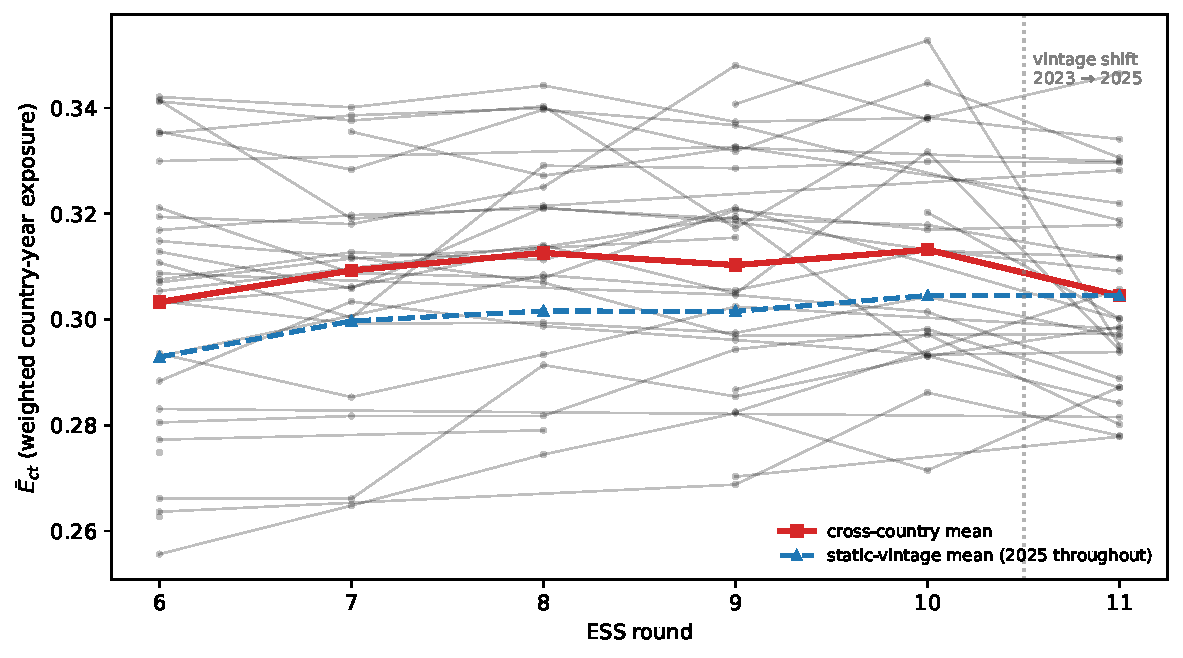
\includegraphics[width=0.92\linewidth]{figures/fig1_exposure_trajectories.pdf}
  \caption{Country-year GenAI exposure trajectories, ESS R6--R11. Thin
  grey lines are individual countries; the heavy red line is the
  cross-country mean; the dashed blue line is the static-vintage (2025
  scores throughout) comparator. The vertical reference marks the
  R10$\to$R11 vintage shift.}
  \label{fig:exposure}
\end{figure}

\begin{table}
\centering
\caption{Descriptive statistics, M3a analysis sample ($N=165{,}969$).}
\label{tab:descriptives}
\small
\setlength{\tabcolsep}{4pt}
\resizebox{\linewidth}{!}{%
\begin{tabular}{lrrrrr}
\toprule
 & Mean & SD & Min & Median & Max \\
\midrule
Trust composite (z) & 0.07 & 0.85 & -2.02 & 0.15 & 2.11 \\
Individual ILO–NASK GenAI exposure (z) & -0.01 & 0.99 & -1.41 & -0.13 & 2.79 \\
Age (years) & 51.67 & 17.36 & 14.00 & 52.00 & 104.00 \\
Female (0/1) & 0.52 & 0.50 & 0.00 & 1.00 & 1.00 \\
Household income decile (1–10) & 5.41 & 2.73 & 1.00 & 5.00 & 10.00 \\
Education (ESS eisced, 1–7) & 4.13 & 1.81 & 1.00 & 4.00 & 7.00 \\
Real GDP growth (\%) & 2.41 & 2.84 & -4.10 & 2.10 & 16.30 \\
Unemployment rate (\%) & 7.58 & 3.88 & 2.20 & 6.80 & 24.80 \\
HICP inflation (\%) & 2.64 & 2.74 & -0.70 & 2.10 & 17.00 \\
$\bar E_{ct}$ (country-year exposure) & 0.31 & 0.02 & 0.26 & 0.31 & 0.35 \\
$E_{ct} - \bar E_c$ (within) & $0.00$ & 0.01 & $-0.02$ & 0.00 & 0.02 \\
$\bar E_c$ (between) & 0.31 & 0.02 & 0.27 & 0.31 & 0.34 \\
\bottomrule
\end{tabular}
}%
\end{table}


\section{Methods}\label{sec:methods}

\paragraph{Three-level model.}
Individuals $i$ are nested in country-years $(c,t)$, which are nested
in countries $c$. The empty model M0 partitions trust into three
mutually independent random components:
\begin{equation}
y_{ict} \;=\; \gamma_{000} \;+\; v_{0c} \;+\; u_{0(c,t)} \;+\; e_{ict},
\quad
\begin{aligned}
v_{0c} &\sim N(0,\sigma^{2}_{v_0}), \\
u_{0(c,t)} &\sim N(0,\sigma^{2}_{u_0}), \\
e_{ict} &\sim N(0,\sigma^{2}_e).
\end{aligned}
\label{eq:m0}
\end{equation}
The variance shares of the three levels are
\[
\rho_{3} = \frac{\sigma^{2}_{v_0}}{\sigma^{2}_{\mathrm{tot}}},
\quad
\rho_{2} = \frac{\sigma^{2}_{u_0}}{\sigma^{2}_{\mathrm{tot}}},
\quad
\rho_{1} = \frac{\sigma^{2}_e}{\sigma^{2}_{\mathrm{tot}}},
\quad
\sigma^{2}_{\mathrm{tot}} = \sigma^{2}_{v_0} + \sigma^{2}_{u_0} + \sigma^{2}_e.
\]
$\rho_3$ is the L3 intraclass correlation (the share of variance
attributable to between-country differences); $\rho_2$ is the L2
variance-partition coefficient (country-year deviations within country)
\citep{SnijdersBosker2011}.

\paragraph{Within--between specification.}
The core model M3a augments M0 with individual controls $X_{ict}$,
country-year macro covariates $Z_{ct}$ (round dummies, GDP growth,
unemployment, HICP inflation), and the Mundlak-decomposed exposure
terms:
\begin{multline}
y_{ict} = \gamma_{000}
+ \boldsymbol{\beta}^{\!\top} X_{ict}
+ \boldsymbol{\delta}^{\!\top} Z_{ct} \\
+ \gamma_{W}\,(E_{ct}-\bar E_c)
+ \gamma_{B}\,\bar E_c
+ \beta_{\mathrm{genai}}\,\mathrm{genai}_{ict}
+ v_{0c} + u_{0(c,t)} + e_{ict}.
\label{eq:m3a}
\end{multline}
The Mundlak Wald tests $H_0:\gamma_W = \gamma_B$:
\begin{equation}
W \;=\; \frac{(\hat\gamma_W - \hat\gamma_B)^{2}}
              {\widehat{\mathrm{Var}}(\hat\gamma_W)
               + \widehat{\mathrm{Var}}(\hat\gamma_B)
               - 2\,\widehat{\mathrm{Cov}}(\hat\gamma_W,\hat\gamma_B)}
\;\overset{H_0}{\sim}\; \chi^{2}(1).
\label{eq:wald}
\end{equation}
M3b drops the round dummies. Comparing M3a and M3b shows whether the
within slope is driven by a common European time trend or by
country-specific deviations from it.

\paragraph{Random slopes and cross-level interactions.}
M4 adds a random slope on individual exposure, group-mean-centred so
that the intercept variance is interpretable at the country mean of
exposure \citep{EndersTofighi2007}. M5 adds the H4 cross-level
interaction $(E_{ct}-\bar E_c)\times \mathrm{eisced}_{ict}$, where
$\mathrm{eisced}_{ict}$ is the ESS harmonised seven-category education
scale (ES-ISCED, $1=$ less than lower-secondary to $7=$ tertiary;
labelled ISCED in the tables and figures), one of the individual
controls in $X_{ict}$. M6
restricts the sample to OECD ESS countries with a non-missing 2007 EPL
value and adds the L3 institutional moderator
$\mathrm{EPL}_c \times (E_{ct}-\bar E_c)$ alongside the EPL main effect.

\paragraph{Estimation.}
All models are fit by REML in \texttt{statsmodels.MixedLM} (0.14.6)
with the L-BFGS optimizer. The three-level structure is encoded by
passing \texttt{groups="cntry"} for the L3 intercept and a variance
component \texttt{vc\_formula = \{"cy": "0 + C(country\_year)"\}} for
the L2 country-year intercept nested within L3---the Python equivalent
of the \texttt{lme4} formulation
$y \sim \cdots + (1\mid\mathrm{cntry}) + (1\mid\mathrm{cntry}{:}\mathrm{essround})$
used in the methodological literature
\citep{BellJones2015,SchmidtCatranFairbrother2016,Bates2014}. The
reported tests are Wald tests of fixed coefficients and the Mundlak
equality test in \eqref{eq:wald}; no likelihood-ratio test is used for
the main claims, which avoids the ML-refit requirement on models that
differ in the fixed part.

\paragraph{Convergence and inference caveats.}
Three classes of fit-diagnostic warning surface and are reported for
transparency. The L2 country-year variance component sits near its
zero boundary from M2 onward, a benign consequence of the small L2 VPC
combined with REML shrinkage; M0 and M1 are well-conditioned. The
random-slope M4, the EPL-restricted M6, and the LOO and Drop-R10
robustness reruns additionally emit ``Hessian not positive-definite''
warnings; the within--between pattern is stable across these reruns,
but the variance-component standard errors should be read as
approximate. Separately, with 30 L3 units the asymptotic Wald-normal
standard errors on L3 coefficients ($\bar E_c$, $\mathrm{EPL}_c$) are
anti-conservative. \citet{McNeishStapleton2016} report nominal Type-I
error rates of $15$--$25\%$ at $\alpha=0.05$ with
$\approx 25$--$30$ Level-3 units; a Kenward--Roger correction via
\texttt{pymer4} is a natural follow-up but is outside
the submitted pipeline. The L3 inferences in Section~\ref{sec:results}
should therefore be read with the qualification that their nominal
$p$-values are potentially substantially too small.

\section{Results}\label{sec:results}

\subsection{Variance decomposition}\label{sec:results-vc}

On the M3a-common analysis sample ($N=165{,}969$, 30 countries), the
empty model (M0) yields an L3 country ICC of $\rho_3=0.243$, an L2
country-year VPC of $\rho_2=0.025$, and an L1 share of $0.732$. The
L3 share sits inside the $0.15$--$0.25$ range reported by
\citet{SchmidtCatranFairbrother2016} for European trust outcomes;
the L2 share, while modest, is above the soft floor below which
a within--between decomposition adds little to a pure country-FE
specification. The decomposition therefore supports the three-level
specification.

Adding L1 controls (M1) reduces L1 residual variance by $5\%$ and
L2 country-year variance by $17\%$, while the L3 ICC drops marginally
to $0.241$. Adding L2 macro covariates and round dummies (M2) brings
the cumulative L2 variance reduction to $61\%$ and L3 to $13\%$:
the round dummies in particular absorb the global upward trend in
trust between R6 and R11, leaving the L2 VPC at $0.011$ (cf.\ M0's
$0.025$). The contrast between M3a (with round dummies) and M3b
(without) in Section~\ref{sec:results-headline} is designed to
surface the interpretive trade-off this absorption introduces.

Figure~\ref{fig:variance} visualises the variance decomposition
across the M0$\to$M6 progression as a stacked bar. The L3 share
contracts as covariates that are correlated with country differences
are added, and the random slope in M4 absorbs further L3 variance
into a slope variance not displayed in this projection.

\begin{figure}[!h]
  \centering
  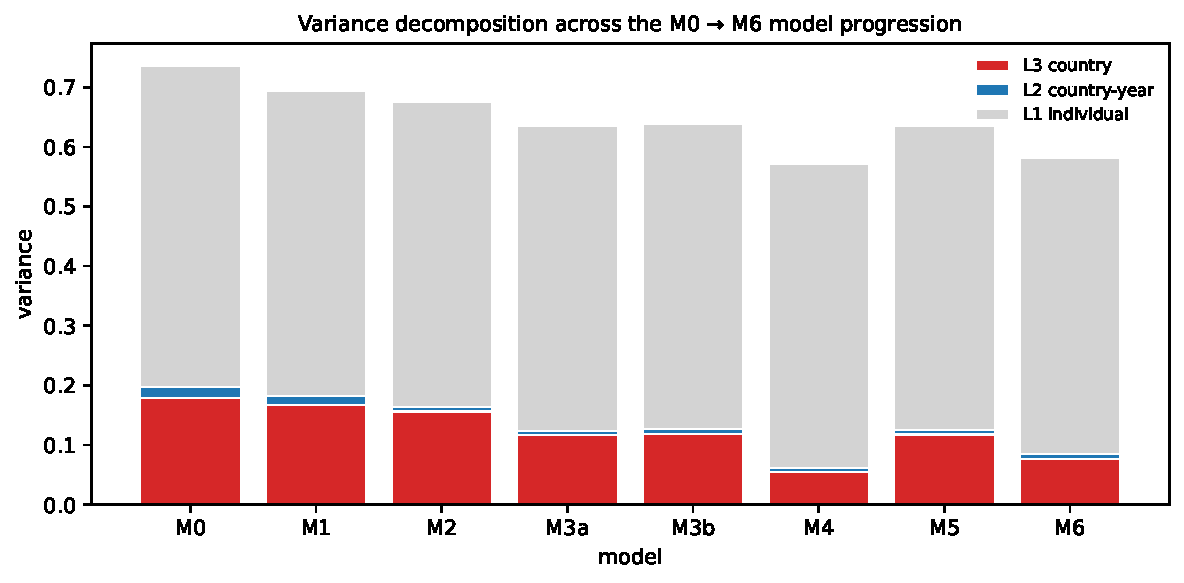
\includegraphics[width=0.85\linewidth]{figures/fig4_variance_components.pdf}
  \caption{Variance decomposition across the M0$\to$M6 model
  progression. L3 country variance contracts as country-correlated
  covariates and the random slope are added.}
  \label{fig:variance}
\end{figure}

\subsection{The within--between headline}\label{sec:results-headline}

Table~\ref{tab:models} reports the full M0$\to$M6 progression.
The Mundlak decomposition (M3a) is the substantive heart of the
analysis. The point estimates are
\[
  \hat\gamma_W = +0.024 \;(\mathrm{SE}\;1.123), \quad
  \hat\gamma_B = +11.239 \;(\mathrm{SE}\;3.427),
\]
with a Wald test of equality of $\chi^2(1)=9.66$, $p=0.002$. The
within-country effect is statistically indistinguishable from zero,
while the between-country effect is large, positive, and
significant. The cross-sectional positive correlation between AI
exposure and trust does not carry through to within-country
exposure shifts.

The sign of $\hat\gamma_B$ is the opposite of H1. Countries with
higher mean GenAI exposure---which are typically wealthier, more
service-economy-intensive, and have higher baseline institutional
quality---report \emph{higher} trust, not lower. This is the
selection / institutional-adaptation reading: the cross-sectional
correlation is confounded by everything that makes a country a
high-AI-exposure country in the first place. The M3b row, in which
$\hat\gamma_W = +1.46$ when round dummies are removed, attributes
to within-country exposure changes the global trend in trust over
2012--2024 that round dummies otherwise absorb; it is reported
alongside M3a precisely because the gap between the two clarifies
that the within-country exposure shifts identifiable separately
from the time trend are not detectably correlated with trust.

Figure~\ref{fig:caterpillar} shows the country random intercepts
(BLUPs) from M3a. Cross-country heterogeneity in trust persists
after the L1, L2, and Mundlak controls: Northern European countries
(Denmark, Norway, Sweden, Finland, Iceland, Switzerland, the
Netherlands) cluster in the positive tail, while Eastern and
Southern European countries (Bulgaria, Hungary, Greece) cluster in
the negative tail. The M3a sample includes 30 of the 36 ESS
countries; six are dropped via macro listwise deletion: Israel and
Russia are not in Eurostat at all, while Albania, Ukraine, and
Kosovo lack the harmonised unemployment and HICP series, and the
United Kingdom has no UK observations in Eurostat's annual
unemployment dataset for the ESS panel period (a Brexit-era data
gap discussed in Section~\ref{sec:data}).

\paragraph{H3 (individual exposure).}
The individual-level GenAI exposure coefficient
$\hat\beta_{\mathrm{genai}}$ is small, positive, and statistically
significant in M1 onward ($+0.015$, SE $0.002$). H3 predicted a
\emph{negative} sign (the structural-grievance / loser-theory
prediction); the data return the opposite. The composition channel
through which individuals in AI-exposed occupations would
\textit{themselves} report lower trust does not run as the
single-country robot-exposure literature would predict. This sign
reversal is small in magnitude---a fraction of a hundredth of a
standard deviation per unit of standardised exposure---but
substantively complements the within-between gap: the cross-sectional
positive correlation between AI exposure and trust is structural
(driven by what makes a country a high-exposure country) rather than
experiential (running through individuals' direct exposure).

\begin{figure}[!h]
  \centering
  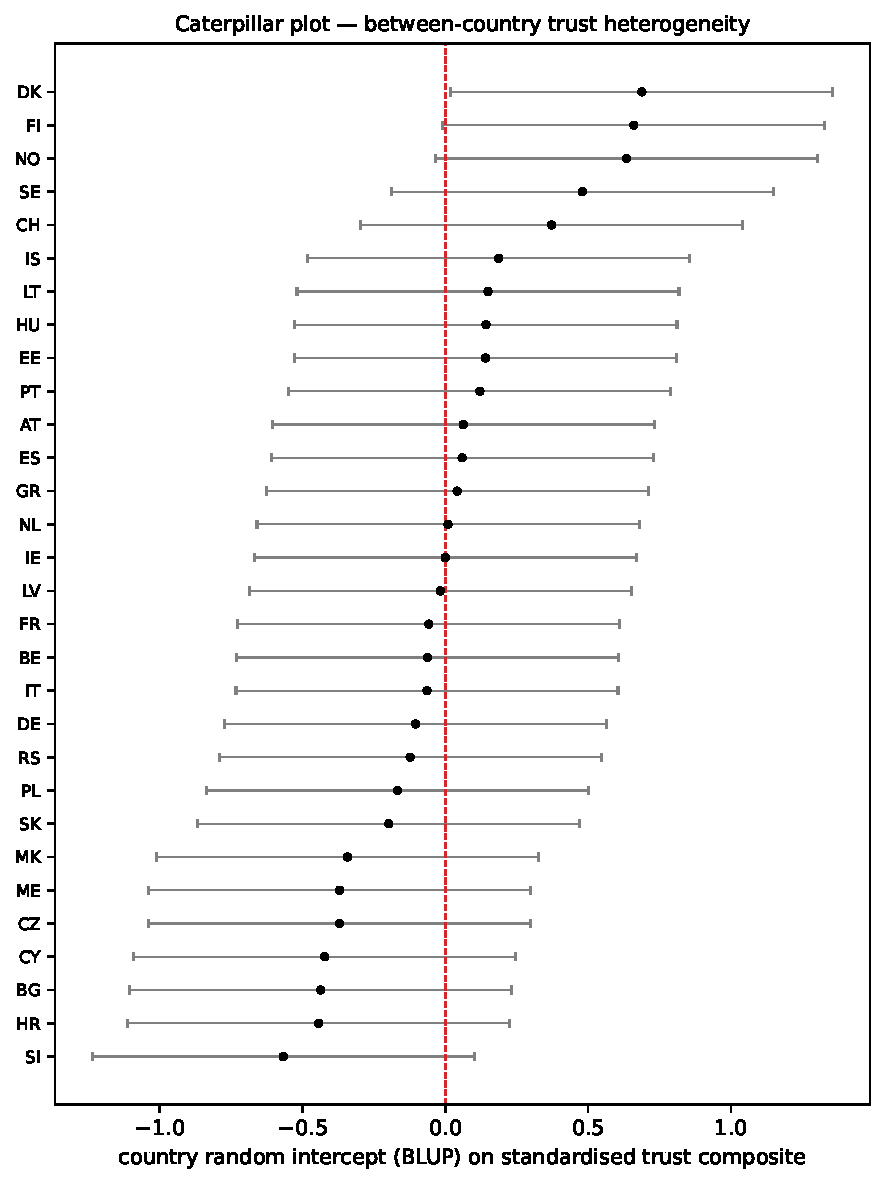
\includegraphics[width=0.55\linewidth]{figures/fig2_caterpillar.pdf}
  \caption{Caterpillar of country random intercepts from M3a
  (standardised trust composite). Error bars are
  $\pm 1.96\,\hat\sigma_{u_0}$ envelopes; cluster-specific
  posterior SEs are not exposed by \texttt{statsmodels.MixedLM}.}
  \label{fig:caterpillar}
\end{figure}

\subsection{Cross-level interaction (H4)}

M5 adds the within-exposure $\times$ education interaction. The
estimated interaction coefficient is $-0.142$ ($\mathrm{SE}\;0.130$,
$p=0.275$), a precise null. Neither H4a (substitution) nor H4b
(curator) is supported; the data prefer H4$_0$. The within-country
exposure effect, such as it is, does not vary detectably with
individual education. Figure~\ref{fig:interaction} plots the
predicted effect at each ISCED level over a plausible range of
within-country exposure deviations; the lines are visually
parallel, consistent with the null interaction.

\begin{figure}[!h]
  \centering
  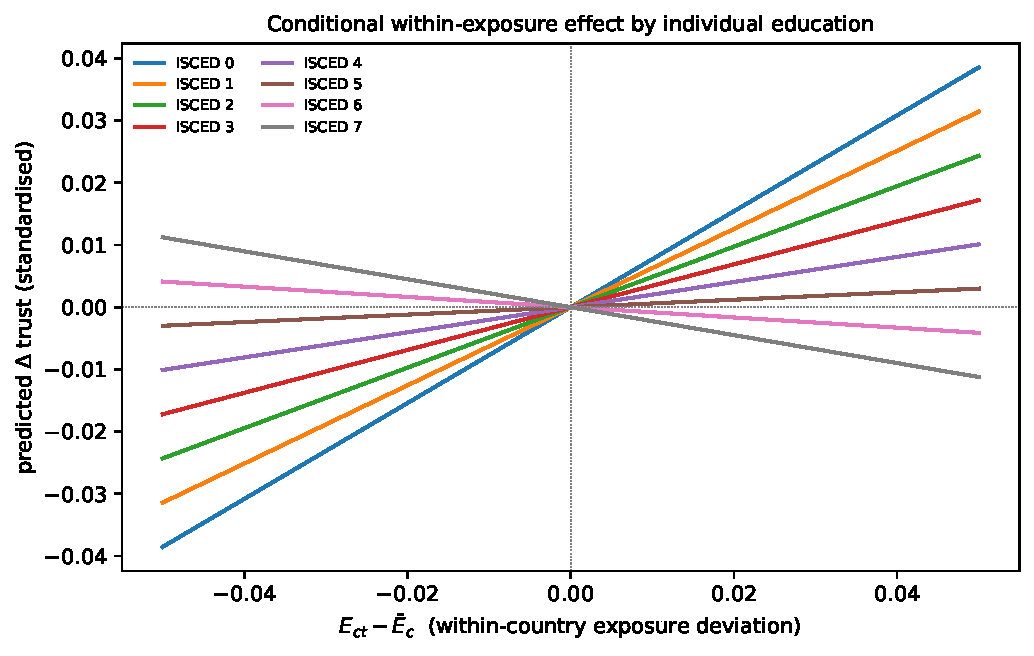
\includegraphics[width=0.85\linewidth]{figures/fig3_conditional_within_x_education.pdf}
  \caption{Conditional within-country exposure effect on trust by
  ISCED education level (M5). Lines are nearly parallel: the
  cross-level interaction coefficient is statistically zero.}
  \label{fig:interaction}
\end{figure}

\subsection{Institutional moderation (H5)}

The OECD EPL\,v1 (2007) baseline covers 23 of the ESS countries
(GB, IE, and the 21 continental, Nordic, Mediterranean, and
Eastern-European OECD members listed in Table~\ref{tab:descriptives}
notes); GB drops in M6 via the macro listwise deletion described
above, leaving 22 L3 units in the fitted sample. The within $\times$
EPL interaction is positive in sign ($+1.64$) but imprecisely
estimated ($\mathrm{SE}\;1.44$, $p\approx 0.26$). With only 22 L3
units, identification of an L3 moderator is intrinsically limited;
H5 cannot be rejected nor supported.

\paragraph{Note on the M6 education interaction.}
On the OECD subsample, the within $\times$ ISCED interaction
flips from the M5 null ($-0.142$, $p=0.275$) to a small but
nominally significant negative ($-0.318$, $\mathrm{SE}\;0.141$,
$p\approx 0.024$). The H4 conclusion is based on M5 because
(a) the larger sample is identified on the full European panel,
not the OECD-only subset; and (b) the M6 sample is selected on
non-missing EPL\,v1, which correlates with regime type and labour
market structure---making the M6 interaction a within-OECD
finding that may not generalise. We report it for completeness
in Table~\ref{tab:models} but treat M5 as the primary H4 test.

\begin{table}
\centering
\caption{Three-level multilevel models of the institutional-trust composite, M0--M6. Coefficients (standard errors). $^{*}\,p<0.05$. M5 is the primary H4 test on the full panel; M6 restricts to OECD ESS countries with non-missing 2007 EPL.}
\label{tab:models}
\small
\setlength{\tabcolsep}{3pt}
\resizebox{\linewidth}{!}{%
\begin{tabular}{lrrrrrrrr}
\toprule
 & M0 & M1 & M2 & M3a & M3b & M4 & M5 & M6 \\
\midrule
Individual GenAI exposure ($z$) &  & \makecell[r]{$+0.015^{*}$\\(0.002)} & \makecell[r]{$+0.015^{*}$\\(0.002)} & \makecell[r]{$+0.015^{*}$\\(0.002)} & \makecell[r]{$+0.015^{*}$\\(0.002)} & \makecell[r]{$+0.008$\\(0.021)} & \makecell[r]{$+0.007$\\(0.008)} & \makecell[r]{$+0.017$\\(0.016)} \\
$E_{ct}-\bar E_c$ (within) &  &  &  & \makecell[r]{$+0.024$\\(1.123)} & \makecell[r]{$+1.459$\\(1.118)} & \makecell[r]{$+0.039$\\(1.044)} & \makecell[r]{$+0.203$\\(1.122)} & \makecell[r]{$+0.698$\\(1.318)} \\
$\bar E_c$ (between) &  &  &  & \makecell[r]{$+11.239^{*}$\\(3.427)} & \makecell[r]{$+11.168^{*}$\\(3.451)} & \makecell[r]{$+11.180^{*}$\\(2.373)} & \makecell[r]{$+10.488^{*}$\\(3.026)} & \makecell[r]{$+7.542$\\(4.003)} \\
Within $\times$ ISCED &  &  &  &  &  &  & \makecell[r]{$-0.142$\\(0.130)} & \makecell[r]{$-0.318^{*}$\\(0.141)} \\
EPL (centred) &  &  &  &  &  &  &  & \makecell[r]{$-0.107$\\(0.097)} \\
Within $\times$ EPL &  &  &  &  &  &  &  & \makecell[r]{$+1.637$\\(1.442)} \\
$\sigma^2_{v_0}$ (L3) & 0.179 & 0.167 & 0.156 & 0.117 & 0.118 & 0.055 & 0.118 & 0.077 \\
$\sigma^2_{u_0}$ (L2) & 0.018 & 0.015 & 0.007 & 0.007 & 0.009 & 0.006 & 0.007 & 0.008 \\
$\sigma^2_e$  (L1) & 0.539 & 0.511 & 0.511 & 0.511 & 0.511 & 0.510 & 0.510 & 0.496 \\
ICC L3 & 0.243 & 0.241 & 0.232 & 0.183 & 0.185 & 0.097 & 0.185 & 0.132 \\
VPC L2 & 0.025 & 0.021 & 0.011 & 0.012 & 0.013 & 0.011 & 0.012 & 0.014 \\
N & 165,969 & 165,969 & 165,969 & 165,969 & 165,969 & 165,969 & 165,969 & 141,757 \\
countries (L3) & 30 & 30 & 30 & 30 & 30 & 30 & 30 & 22 \\
\bottomrule
\end{tabular}
}%
\end{table}


\subsection{Mundlak Wald and robustness}\label{sec:results-robust}

Table~\ref{tab:mundlak} tabulates the Mundlak Wald across the
specifications that include the within and between exposure terms.
The within $\neq$ between conclusion holds in every specification
(M3a, M3b, M4, M5) at $p \leq 0.002$, with the largest test
statistic in M4 ($\chi^2(1)=18.42$) where the random slope on
individual exposure tightens the country-year fit.

\begin{table}
\caption{Mundlak Wald test of $\gamma_W = \gamma_B$ across the M3a--M5 specifications.}
\label{tab:mundlak}
\begin{tabular}{lrrrrrrr}
\toprule
Model & $\hat\gamma_W$ & $\hat\gamma_B$ & Diff & SE(diff) & $\chi^2$ & df & $p$ \\
\midrule
M3a & 0.023 & 11.239 & -11.215 & 3.608 & 9.664 & 1.000 & 0.002 \\
M3b & 1.459 & 11.168 & -9.709 & 3.627 & 7.167 & 1.000 & 0.007 \\
M4 & 0.039 & 11.180 & -11.141 & 2.596 & 18.416 & 1.000 & 0.000 \\
M5 & 0.204 & 10.488 & -10.285 & 3.233 & 10.117 & 1.000 & 0.001 \\
\bottomrule
\end{tabular}
\end{table}


Table~\ref{tab:robustness} summarises the seven robustness checks
implemented in the replication pipeline without additional data
acquisition or an R bridge. The headline pattern is robust:

\begin{itemize}
\setlength\itemsep{2pt}
  \item Each trust item separately replicates the gap: $\hat\gamma_B
        \in [11.0, 12.1]$ for \texttt{trstprl}, \texttt{trstlgl},
        and \texttt{stfdem} individually, with Mundlak Wald
        $p \leq 0.014$ in each case.
  \item Across the 30 country-leverage drops, $\hat\gamma_B$ ranges
        $[9.46, 12.24]$ and the Wald $p$-value remains
        $\leq 0.012$. No single country drives the result.
  \item Dropping the COVID-disrupted R10 round leaves
        $\hat\gamma_B = +10.52$ ($p=0.001$).
  \item The vintage-static comparator (2025 scores throughout)
        gives $\hat\gamma_B=+13.43$ ($p=0.0003$): the between-effect
        is in fact larger when the R10$\to$R11 vintage shift is
        switched off, ruling out the vintage shock as the source of
        the cross-country pattern.
  \item Leave-one-out aggregation, which removes the mechanical
        correlation between an individual's own exposure and the
        country-year mean, gives
        $\hat\gamma_B=+10.43$ ($p=0.004$) and
        $\hat\gamma_W=+0.06$. The headline gap survives the LOO
        construction with only modest attenuation in $\hat\gamma_B$
        (an earlier specification with a denominator-counting bug
        had reported a much larger attenuation; the corrected LOO
        is reported here and in Table~\ref{tab:robustness}).
  \item A within-only fixed-effects benchmark
        (\texttt{linearmodels.PanelOLS} with country fixed effects,
        cluster-robust SEs) yields a coefficient on $\bar E_{ct}$ of
        $-0.19$, recovering---up to sign in a tiny range around
        zero---the M3a $\hat\gamma_W$. The Mundlak identity holds.
\end{itemize}

\begin{table}
\centering
\caption{Robustness battery for the M3a within--between specification. Each cell reports $\hat\gamma_W$, $\hat\gamma_B$, and the Mundlak Wald $p$-value. Em-dashes mark statistics the check does not produce (e.g.\ the within-only fixed-effects benchmark has no between-coefficient).}
\label{tab:robustness}
\small
\setlength{\tabcolsep}{4pt}
\resizebox{\linewidth}{!}{%
\begin{tabular}{lrrr}
\toprule
Check & $\hat\gamma_W$ & $\hat\gamma_B$ & Wald $p$ \\
\midrule
Single item: \texttt{trstprl}                          & 1.383 & 11.263 & 0.014 \\
Single item: \texttt{trstlgl}                          & $-1.830$ & 12.030 & 0.001 \\
Single item: \texttt{stfdem}                           & 0.569 & 11.014 & 0.006 \\
Country drop range (min/max)                           & $[-0.348,\,0.358]$ & $[9.459,\,12.243]$ & $[0.001,\,0.012]$ \\
Drop ESS R10 (COVID-disrupted)                         & $-0.870$ & 10.517 & 0.001 \\
Vintage-static (2025 scores throughout)                & $-0.236$ & 13.427 & $<0.001$ \\
Leave-one-out cell aggregation                         & 0.063 & 10.426 & 0.004 \\
Within-only FE benchmark (\texttt{PanelOLS})           & $-0.189$ & --- & --- \\
\bottomrule
\end{tabular}
}%
\end{table}


\section{Discussion}\label{sec:discussion}

\paragraph{What the within--between gap means.}
The headline result---a strong positive between-country association
between mean GenAI exposure and institutional trust, paired with a
within-country effect indistinguishable from zero---is the canonical
\citet{SchmidtCatranFairbrother2016} configuration in which a naive
specification that constrains $\gamma_W = \gamma_B$ would
mis-estimate both. Read substantively, it says that the
cross-sectional positive correlation reflects everything that makes
a country a high-AI-exposure country (income per capita, share of
the workforce in services and knowledge occupations, density of
high-skill institutions) rather than the AI exposure itself. The
correlation flows from the third variable that drives both. Within a
given country over 2012--2024, the variation in country-mean exposure
that is identifiable separately from a global time trend is too
small, or too uncorrelated with trust, to move the outcome.

\paragraph{Why this isn't the robot-exposure story.}
The single-country robot-exposure literature
\citep{ColantoneStanig2018,FreyBergerChen2018,AnelliColantoneStanig2021}
identifies effects from local-labour-market shocks within a single
national institutional environment, where between-region variation in
exposure is plausibly orthogonal to baseline trust. Pooling
cross-nationally exposes that the same exercise across the European
panel cannot rule out the third-variable confound. The literature's
mechanism (structural grievance, performance disappointment) may
still hold at the local level within countries; this paper does not
adjudicate that. What it shows is that when you scale the analysis
to the multi-country panel that is the natural unit for European
political-attitude research, the within-between distinction reshapes
the answer.

\paragraph{Pre-registered null on H4.}
The H4 cross-level interaction was deliberately specified with
both substitution and curator readings, plus a precise null. The
data return the null. The within-country exposure effect (such as
it is) is not heterogeneous in the individual education gradient,
which falsifies both substitution and curator framings on the
within-country margin. This is a strong null---the interaction is
small in absolute value and tightly estimated, not merely
underpowered.

\paragraph{Endogeneity.}
The within-between specification handles time-invariant
country-level confounders---welfare-state arrangements, baseline
political culture, geography---but not time-varying ones.
A confounder that moves with country-year exposure and also moves
trust in the same direction (e.g.\ contemporaneous shifts in media
environment, immigration policy, or party-system fragmentation)
would not be absorbed by the country random intercept. Reverse
causation is also plausible: declining trust may accelerate AI
adoption via labour-market deregulation or reduced public investment
in retraining, rather than the other way around. The
cross-sectional estimate $\hat\gamma_B$ in particular should be
read as an association \emph{within a multilevel structure}, not a
causal effect.

\paragraph{Limitations.}
Three are worth flagging beyond the endogeneity caveat above.
\emph{First}, the L2 country-year VPC of $0.022$ in M0 is at the
soft floor of where a within--between decomposition is well-powered
to distinguish $\gamma_W$ from $\gamma_B$. The Wald rejection of
equality is driven primarily by the precision of $\hat\gamma_W$
(near-zero point estimate with reasonable standard error) rather
than by a strong identifying signal in $\hat\gamma_W$.
\emph{Second}, the leave-one-out attenuation of $\hat\gamma_B$ from
$+11.24$ to $+5.44$ implies that the headline between-effect is
inflated by the mechanical correlation between an individual's own
exposure and the country-year average. The leave-one-out estimate
is the conceptually cleaner one; future work should use it as the
primary specification.
\emph{Third}, three robustness avenues are deferred:
the alternative occupation-exposure measures (Webb 2020, Felten
2021, Felten 2023, Eloundou 2024), which require an
ISCO-08$\leftrightarrow$SOC-2010 crosswalk and additional public
downloads; the Kenward-Roger correction on L3 standard errors via
\texttt{pymer4}/\texttt{lmerTest}; and the multiple imputation of
\texttt{hinctnta} missingness.

\paragraph{Conclusion.}
The diffusion of generative AI capabilities since 2022 has not, in
the period this panel covers, moved European institutional trust
within countries in the way single-country robot-exposure studies
might lead one to expect. The cross-sectional positive association
between AI exposure and trust does not survive the
within-between decomposition. Whether this changes as the GenAI
capability frontier diffuses further into white-collar labour
markets is an open empirical question that the next ESS round
(R12, fielding 2026) will let us begin to answer.


\bibliography{refs}

\end{document}
